\documentclass[11pt]{article}
\usepackage[T1]{fontenc}
\usepackage[utf8]{inputenc}
\usepackage[letterpaper]{geometry}

\usepackage{graphicx}
\usepackage{mathpazo}

\usepackage{amsmath}
\usepackage{amsfonts}
\usepackage{bm}
\usepackage{siunitx}
\usepackage{cancel}
\usepackage{float}
\usepackage{empheq}
\usepackage[most]{tcolorbox}
\usepackage{subcaption}

% Sexy yellow highlighted boxed equations!
\newtcbox{\mymath}[1][]{%
  nobeforeafter, math upper, tcbox raise base,
  enhanced, colframe=black!30!black,
  colback=yellow!30, boxrule=1pt,
  #1}

% Hyperlinks with decent looking default colors.
\usepackage{hyperref}
\usepackage{xcolor}
\hypersetup{
  colorlinks,
  linkcolor={red!50!black},
  citecolor={blue!50!black},
  urlcolor={blue!80!black}
}

% For those sexy spaced low small caps from classic-thesis!
\usepackage{microtype}
\usepackage{textcase}
\DeclareRobustCommand{\spacedlowsmallcaps}[1]{%
  \textls[80]{\scshape\MakeTextLowercase{#1}}%
}

% Replaced mathpazo \sum symbol with computer modern's.
\DeclareSymbolFont{cmlargesymbols}{OMX}{cmex}{m}{n}
\let\sumop\relax
\DeclareMathSymbol{\sumop}{\mathop}{cmlargesymbols}{"50}

% Force indent command.
\newcommand{\forceindent}{\leavevmode{\parindent=1em\indent}}

% Math shortcuts.
\newcommand\p[2]{\frac{\partial #1}{\partial #2}}
\newcommand{\norm}[1]{\left\lVert#1\right\rVert}

% fancyhdr header and footer.
\usepackage{fancyhdr}
\pagestyle{fancy} 
\fancyhead{}
\rhead{Ali Ramadhan}
\lhead{6.339 Project 4---Boundary Element Methods}
\cfoot{\thepage}

\title{\spacedlowsmallcaps{6.339: Numerical Methods for Partial Differential Equations}\\ \spacedlowsmallcaps{Project four: Boundary Element Methods}}
\author{Ali Ramadhan$^\text{†}$ (\href{mailto:alir@mit.edu}{\texttt{alir@mit.edu}})}
\date{\textit{$^\text{†}$Department of Earth, Atmospheric, and Planetary Sciences}}

\renewcommand\thesubsection{\thesection(\alph{subsection})}

\begin{document}
\maketitle

\section{Gaussian quadrature using the trapezoidal rule}

\subsection{Derivation of the trapezoidal rule error formula}
We wish to derive a formula, or rather, an upper bound on the error in approximating an integral
\begin{equation}
  I[f] = \int_a^b f(x) \, dx
\end{equation}
via the composite trapezoidal rule
\begin{equation}
  \int_a^b f(x) \, dx \approx \frac{b-a}{n} \left[ \frac{f(a) + f(b)}{2} + \sumop_{i=1}^{n-1} f \left( a + i\frac{b-a}{n} \right) \right]
\end{equation}

We will begin by rewriting the composite trapezoidal rule slightly. Let us define
\begin{equation}
  x_i = a + i \frac{b-a}{n}
\end{equation}
so that $x_0 = a$ and $x_n = b$. Then
\begin{equation*}
 \frac{f(a) + f(b)}{2} + \sumop_{i=1}^{n-1} f \left( a + i\frac{b-a}{n} \right)
  = \frac{f(x_0) + f(x_n)}{2} + \sumop_{i=1}^{n-1} f \left( x_i \right)
  = \sumop_{i=1}^{n} \frac{f(x_{i-1}) + f(x_i)}{2}
\end{equation*}
and we can rewrite the composite trapezoidal rule as
\begin{equation}
\int_a^b f(x) \, dx \approx \frac{b-a}{2n} \sumop_{i=1}^{n} \left[ f(x_{i-1}) + f(x_i) \right]
\end{equation}

The error is then given by
\begin{multline*}
  E[f] = \left\lvert \frac{b-a}{2n} \sumop_{i=1}^n \left[ f(x_{i-1}) + f(x_i) \right] - \int_a^b f(x) \, dx \right\rvert \\
  = \left\lvert \sumop_{i=1}^n \left\{ \frac{b-a}{2n} \left[ f(x_{i-1}) + f(x_i) \right] - \int_{x_i}^{x_{i+1}} f(x) \, dx \right\} \right\rvert
  = \left\lvert \sumop_{i=1}^n E_i[f] \right\rvert
\end{multline*}
where we split up the integral into $n$ integrals, one over each subinterval $x \in [x_{i}, x_{i+1}]$. We let $c_i = (x_{i} + x_{i+1})/2$ denote the midpoint of the $n^\mathrm{th}$ subinterval. We notice that $(b-a)/n$ is the length of one subinterval and so $(b-a)/2n$ must be the length from the beginning of the interval $x_i$ to the midpoint $c_i$:
\begin{equation*}
  x_{i+1} - c_i = x_{i+1} - \frac{x_{i} + x_{i+1}}{2} = \frac{x_{i+1} - x_i}{2}
  = \frac{1}{2} \left[ a + (i+1)\frac{b-a}{n} - \left( a + i\frac{b-a}{n} \right) \right]
  = \frac{b-a}{2n}
\end{equation*}
Then each term in the sum can be written as
\begin{equation*}
  E_i[f]
  = \frac{b-a}{2n} \left[ f(x_{i-1}) + f(x_i) \right] - \int_{x_i}^{x_{i+1}} f(x) \, dx
  = (x_{i+1} - c_i) \left[ f(x_{i-1}) + f(x_i) \right] - \int_{x_i}^{x_{i+1}} f(x) \, dx
\end{equation*}
At this point we realize we can perform an integration by parts in the reverse direction as 
\begin{multline*}
  \int_{x_i}^{x_{i+1}} (x-c_i) f'(x) \, dx
  = (x-c_i)f(x) \Big\rvert_{x_i}^{x_{i+1}} - \int_{x_i}^{x_{i+1}} f(x) \, dx \\
  = (x_{i+1}-c_i)f(x_{i+1}) - (x_i-c_i)f(x_i) - \int_{x_i}^{x_{i+1}} f(x) \, dx \\
  = (x_{i+1}-c_i)f(x_{i+1}) + (x_{i+1}-c_i)f(x_i) - \int_{x_i}^{x_{i+1}} f(x) \, dx \\
  = (x_{i+1}-c_i)\left[ f(x_{i+1}) + f(x_i) \right] - \int_{x_i}^{x_{i+1}} f(x) \, dx
\end{multline*}
where we used the fact that $x_i - c_i = c_i - x_{i+1} = - (x_{i+1} - c_i)$. Therefore the error over the $n^\mathrm{th}$ subinterval can be written as
\begin{equation*}
  E_i[f] = \int_{x_i}^{x_{i+1}} (x-c_i) f'(x) \, dx
\end{equation*}

\subsection{Implementation of the composite trapezoidal rule}
Implementing the composite trapezoidal rule in MATLAB, we can use it to approximate integrals. We will investigate its accuracy in approximating the following four analytically integrable integrals
\begin{align*}
  & \mathrm{(i)} \int_2^{10} 3x \, dx = 144, \quad
    & \mathrm{(ii)} & \int_0^\pi \sin x \, dx = 2 \\
  & \mathrm{(iii)} \int_0^1 e^{2\cos(2\pi x)} \, dx = I_0(2), \quad
    & \mathrm{(iv)}&  \int_0^{2\pi} |\cos x| \, dx = 4
\end{align*}
where $I_\nu(z)$ denotes the modified Bessel function of the first kind. We attempt to approximate the value of the definite integrals using $n=1,2,\dots,100$ subintervals.

\begin{figure}[!htb]
  \centering
  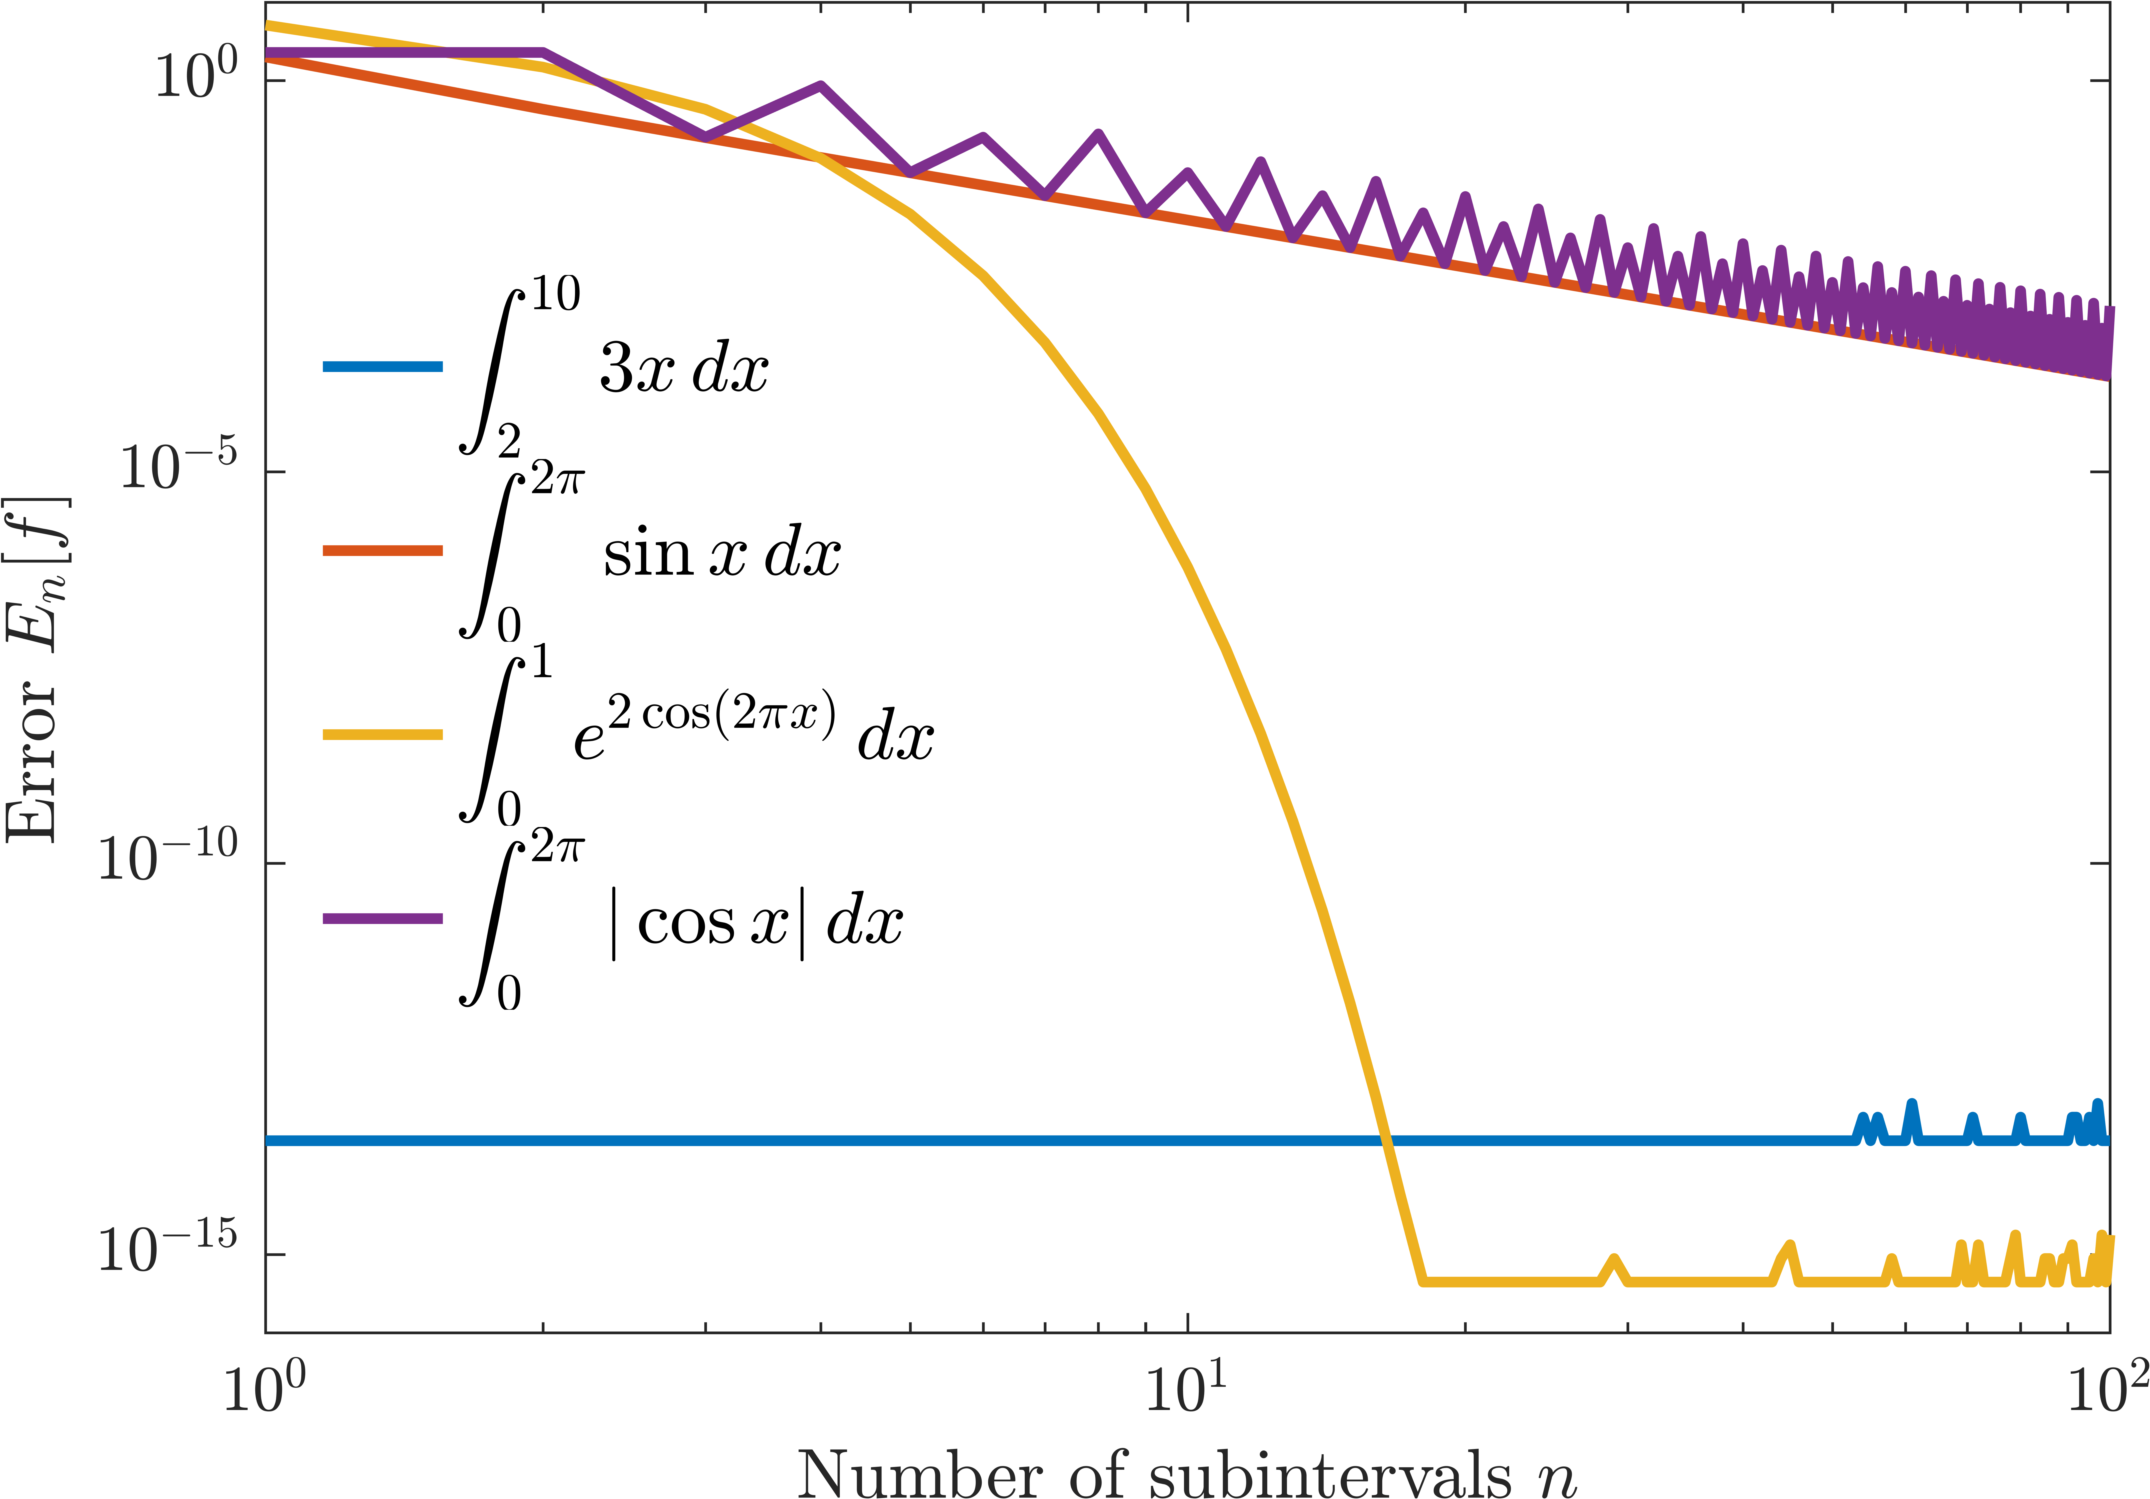
\includegraphics[width=\linewidth]{trapezoid_error.png}
  \caption{The absolute error $E_n[f]$ between the exact integral and the value approximated using the composite trapezoidal rule as a function of the number of subintervals $n$ for the four different integrals labeled in the legend.}
  \label{fig:trapezoid_error}
\end{figure}

Figure \ref{fig:trapezoid_error} shows the absolute error $E_n[f]$ between the approximated integral and the approximated value. We see that the trapezoidal rule is exact for integral (i) no matter the number of subintervals. This is because the trapezoidal rule is exact for any function whose second derivative $f''(x) = 0$ everywhere, which includes first-order polynomials such as $3x$.

For integral (ii) the composite trapezoidal rule seems to converge quadratically as $n$ is increased, as we expect since the error scales as $n^{-2}$. The same can be said for integral (iv) however it exhibits an oscillatory behavior due to the undefined nature of the derivative of the absolute value function at $x=\pi/2$ and $x=3\pi/2$ causing the composite trapezoidal rule to successively overestimate then underestimate the integral each time $n$ is incremented.

For integral (iv) the convergence is exponential or spectral.

\section{Using the Nyström method to solve Laplace's equation}

\subsection{Solving the exterior Neumann problem}
Taking the boundary to be the unit circle $\Gamma = \{(x,y) : \sqrt{x^2 + y^2} = 1\}$ with the Neumann boundary condition on the boundary being
\begin{equation}
  \left. \p{u}{\bm{n}} \right\rvert_\Gamma =  \frac{1}{3 + 2\cos\theta + \cos(2\theta)}
\end{equation}
where $\theta \in [-\pi, \pi]$, $x = \cos\theta$, and $y = \sin\theta$. For the exterior Neumann problem, the monopole integral formulation is given by
\begin{equation}
  \p{u_\Gamma(\bm{x})}{\bm{n}(\bm{x})}
  = -\pi\sigma(\bm{x}) - \mathrm{P.V.}\int_\Gamma \frac{\bm{x-x'}}{\norm{\bm{x-x'}}^2} \cdot \bm{n}(\bm{x}) \, \sigma(\bm{x}') \, d\Gamma'
\end{equation}

Choosing $n$ equally collocation points $\{\theta_i\}_{i=1}^n$ on the boundary and discretizing the integral using a Gaussian quadrature scheme with evaluation points chosen to coincide with the collocation points, we get
\begin{multline*}
  \frac{1}{3 + 2\cos\theta_i + \cos(2\theta_i)}
  = -\pi\sigma(\bm{x}_i) - \mathrm{P.V.}\int_\Gamma \frac{\bm{x_i}-\bm{x}'}{\norm{\bm{x_i}-\bm{x}'}^2} \cdot \bm{n}(\bm{x}) \, \sigma(\bm{x}') \, d\Gamma' \\
  = -\pi \sigma_i - \sumop_{j=1}^n w_j \frac{\bm{x_i}-\bm{x}_j}{\norm{\bm{x_i}-\bm{x}_j}^2} \cdot \bm{n}(\bm{x}_i) \, \sigma_j  \, , \quad i = 1,2,\dots,n 
\end{multline*}
where $\bm{x}_i = (\cos\theta_i, \sin\theta_i)$, $\mathrm{P.V.}$ denotes the Cauchy principal value of the integral, $w_j$ are the quadrature weights, $\sigma(\bm{x}_i) \equiv \sigma_i$ so that $\bm{\sigma}$ denotes the discrete version of $\sigma(\bm{x})$, and $\bm{n}(\bm{x}) = (n_x, n_y) = (\cos\theta, \sin\theta)$ denotes the unit normal vector pointing out of the boundary.

Taking $\bm{x}_i = (\cos\theta, \sin\theta)$, we see that
\begin{multline*}
  \norm{\bm{x_i}-\bm{x}_j}^2
  = (\cos\theta_i - \cos\theta_j)^2 + (\sin\theta_i - \sin\theta_j)^2 \\
  = \cos^2\theta_i - 2\cos\theta_i\cos\theta_j + \cos^2\theta_j + \sin\theta_j + \sin^2\theta_i - 2\sin\theta_i\sin\theta_j + \sin^2\theta_j \\
   = 2(1 - \cos\theta_i\cos\theta_j - \sin\theta_i\sin\theta_j)
\end{multline*}
as $\sin^2\vartheta + \cos^2\vartheta = 1$. The dot product becomes
\begin{equation*}
  (\bm{x}_i - \bm{x}_j) \cdot \bm{n}(\bm{x}_i)
  = (\cos\theta_i - \cos\theta_j)\cos\theta_i + (\sin\theta_i - \sin\theta_j)\sin\theta_i
  = 1 - \cos\theta_i\cos\theta_j - \sin\theta_i\theta_j
\end{equation*}
which is exactly half the denominator ans so we get that
\begin{equation*}
  \frac{\bm{x_i}-\bm{x}_j}{\norm{\bm{x_i}-\bm{x}_j}^2} \cdot \bm{n}(\bm{x}_i)
  = \frac{1 - \cos\theta_i\cos\theta_j - \sin\theta_i\theta_j}{2(1 - \cos\theta_i\cos\theta_j - \sin\theta_i\theta_j)}
  = \frac{1}{2}
\end{equation*}
even for the self term ($i=j$) where $\theta_i \rightarrow \theta_j$ as the numerator and denominator both go to zero at the same rate. The discretized problem becomes a system of $n$ linear equations 
\begin{equation*}
  \frac{1}{3 + 2\cos\theta_i + \cos(2\theta_i)}
  = -\pi\sigma_i - \sumop_{j=1}^n \frac{w_j}{2} \sigma_j \, , \quad i = 1,2,\dots,n
\end{equation*}
where we are interested in solving for $\bm{\sigma} = (\sigma_1, \sigma_2, \dots, \sigma_n)$.

The problem may be easily solved by casting it as a matrix equation $A\bm{\sigma} = \bm{b}$ where
\begin{equation*}
  A_{ii} = -\pi, \quad
  A_{ij} = \frac{w_j}{2} = \frac{\pi}{n}, \quad
  b_i = \frac{1}{3 + 2\cos\theta_i + \cos(2\theta_i)}
\end{equation*}
where we took equal quadrature weights in accordance with the midpoint rule such that $w_j = 2\pi/n$.

\begin{figure}[!htb]
  \centering
  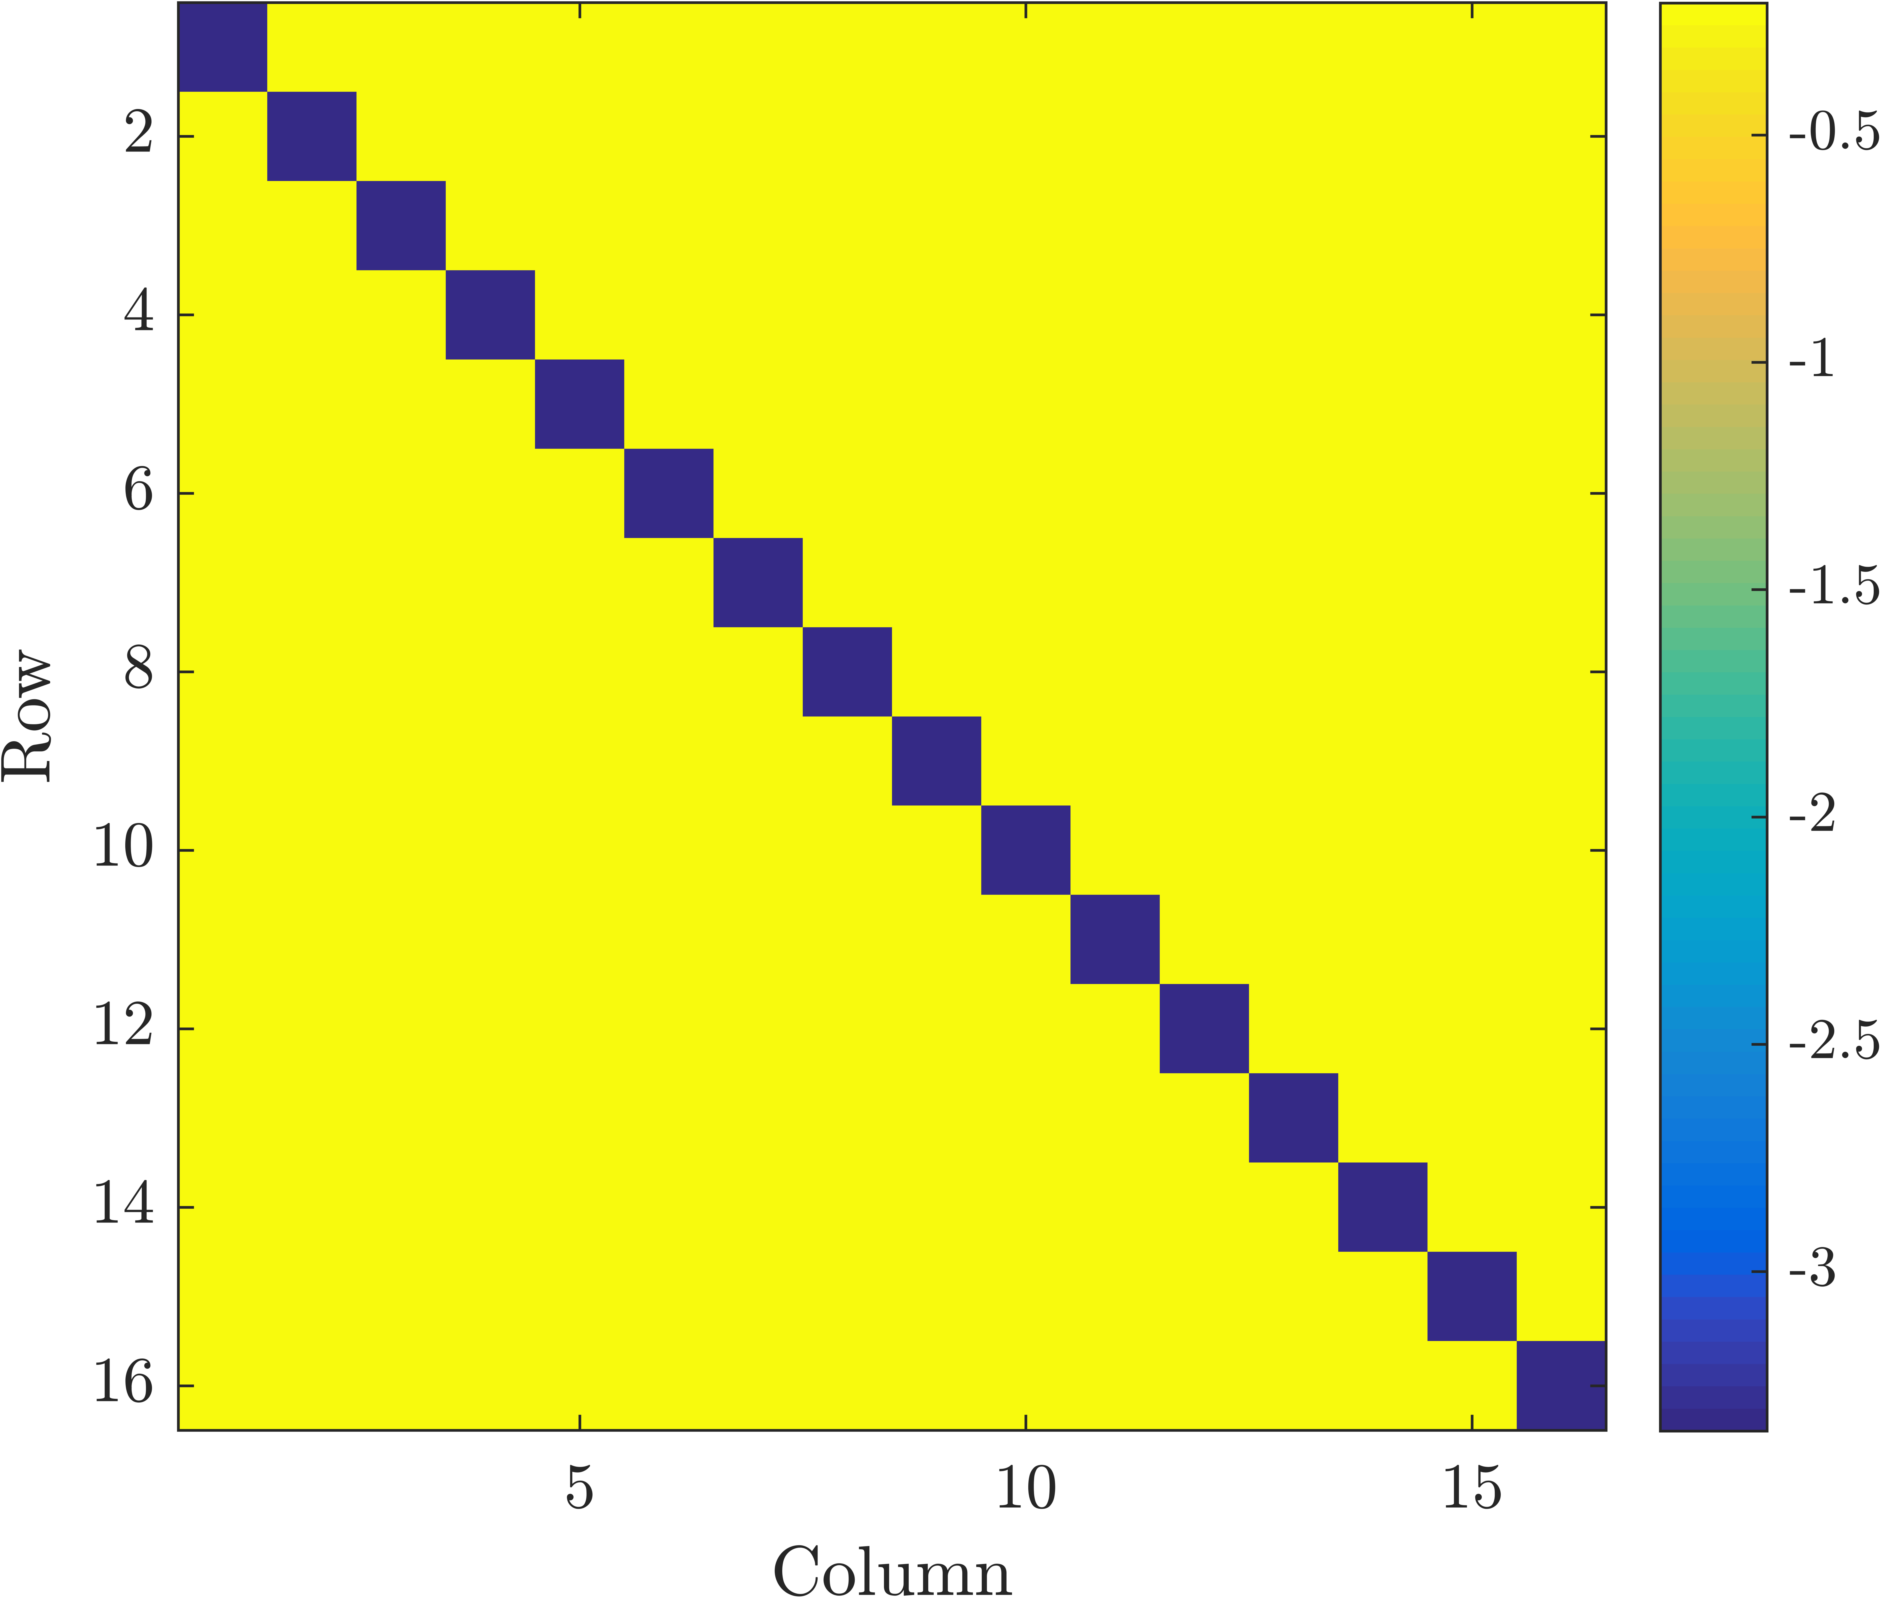
\includegraphics[width=0.7\linewidth]{matrix_heatmap.png}
  \caption{Heatmap of the elements of the $A$ matrix used to solve for $\bm{\sigma}$ via $A\bm{\sigma} = \bm{b}$.}
  \label{fig:matrix_heatmap}
\end{figure}

The magnitude of the elements of the $A$ matrix are shown as a heatmap in figure \ref{fig:matrix_heatmap}. We notice the diagonal contains the largest elements, and indeed the matrix is diagonally dominant as
\begin{equation*}
A_{ii} = |-\pi| > (n-1)\left\lvert \frac{\pi}{n} \right\rvert = \sumop_{j\ne i} |A_{ij}|
\end{equation*}
but just barely. The matrix is full and the off-diagonal elements are small, and all equal.

We are given the exact solution as
\begin{equation}
  \sigma(\theta) = -\frac{1}{\pi} \left( \frac{I}{2} + f(\theta) \right), \quad \theta \in [-\pi, \pi]
\end{equation}
where 
\begin{equation}
  f(\theta) = \frac{1}{3 + 2\cos\theta + \cos(2\theta)}
\end{equation}
and
\begin{equation*}
  I = - \frac{1}{2\pi} \int_{-\pi}^\pi f(\theta) \, d\theta
  = -\frac{1}{6} \sqrt{3 + 2\sqrt{3}}
\end{equation*}
where the integral was evaluated using Mathematica. Using this we can compare our solution with the exact solution.

\begin{figure}[!htb]
  \centering
  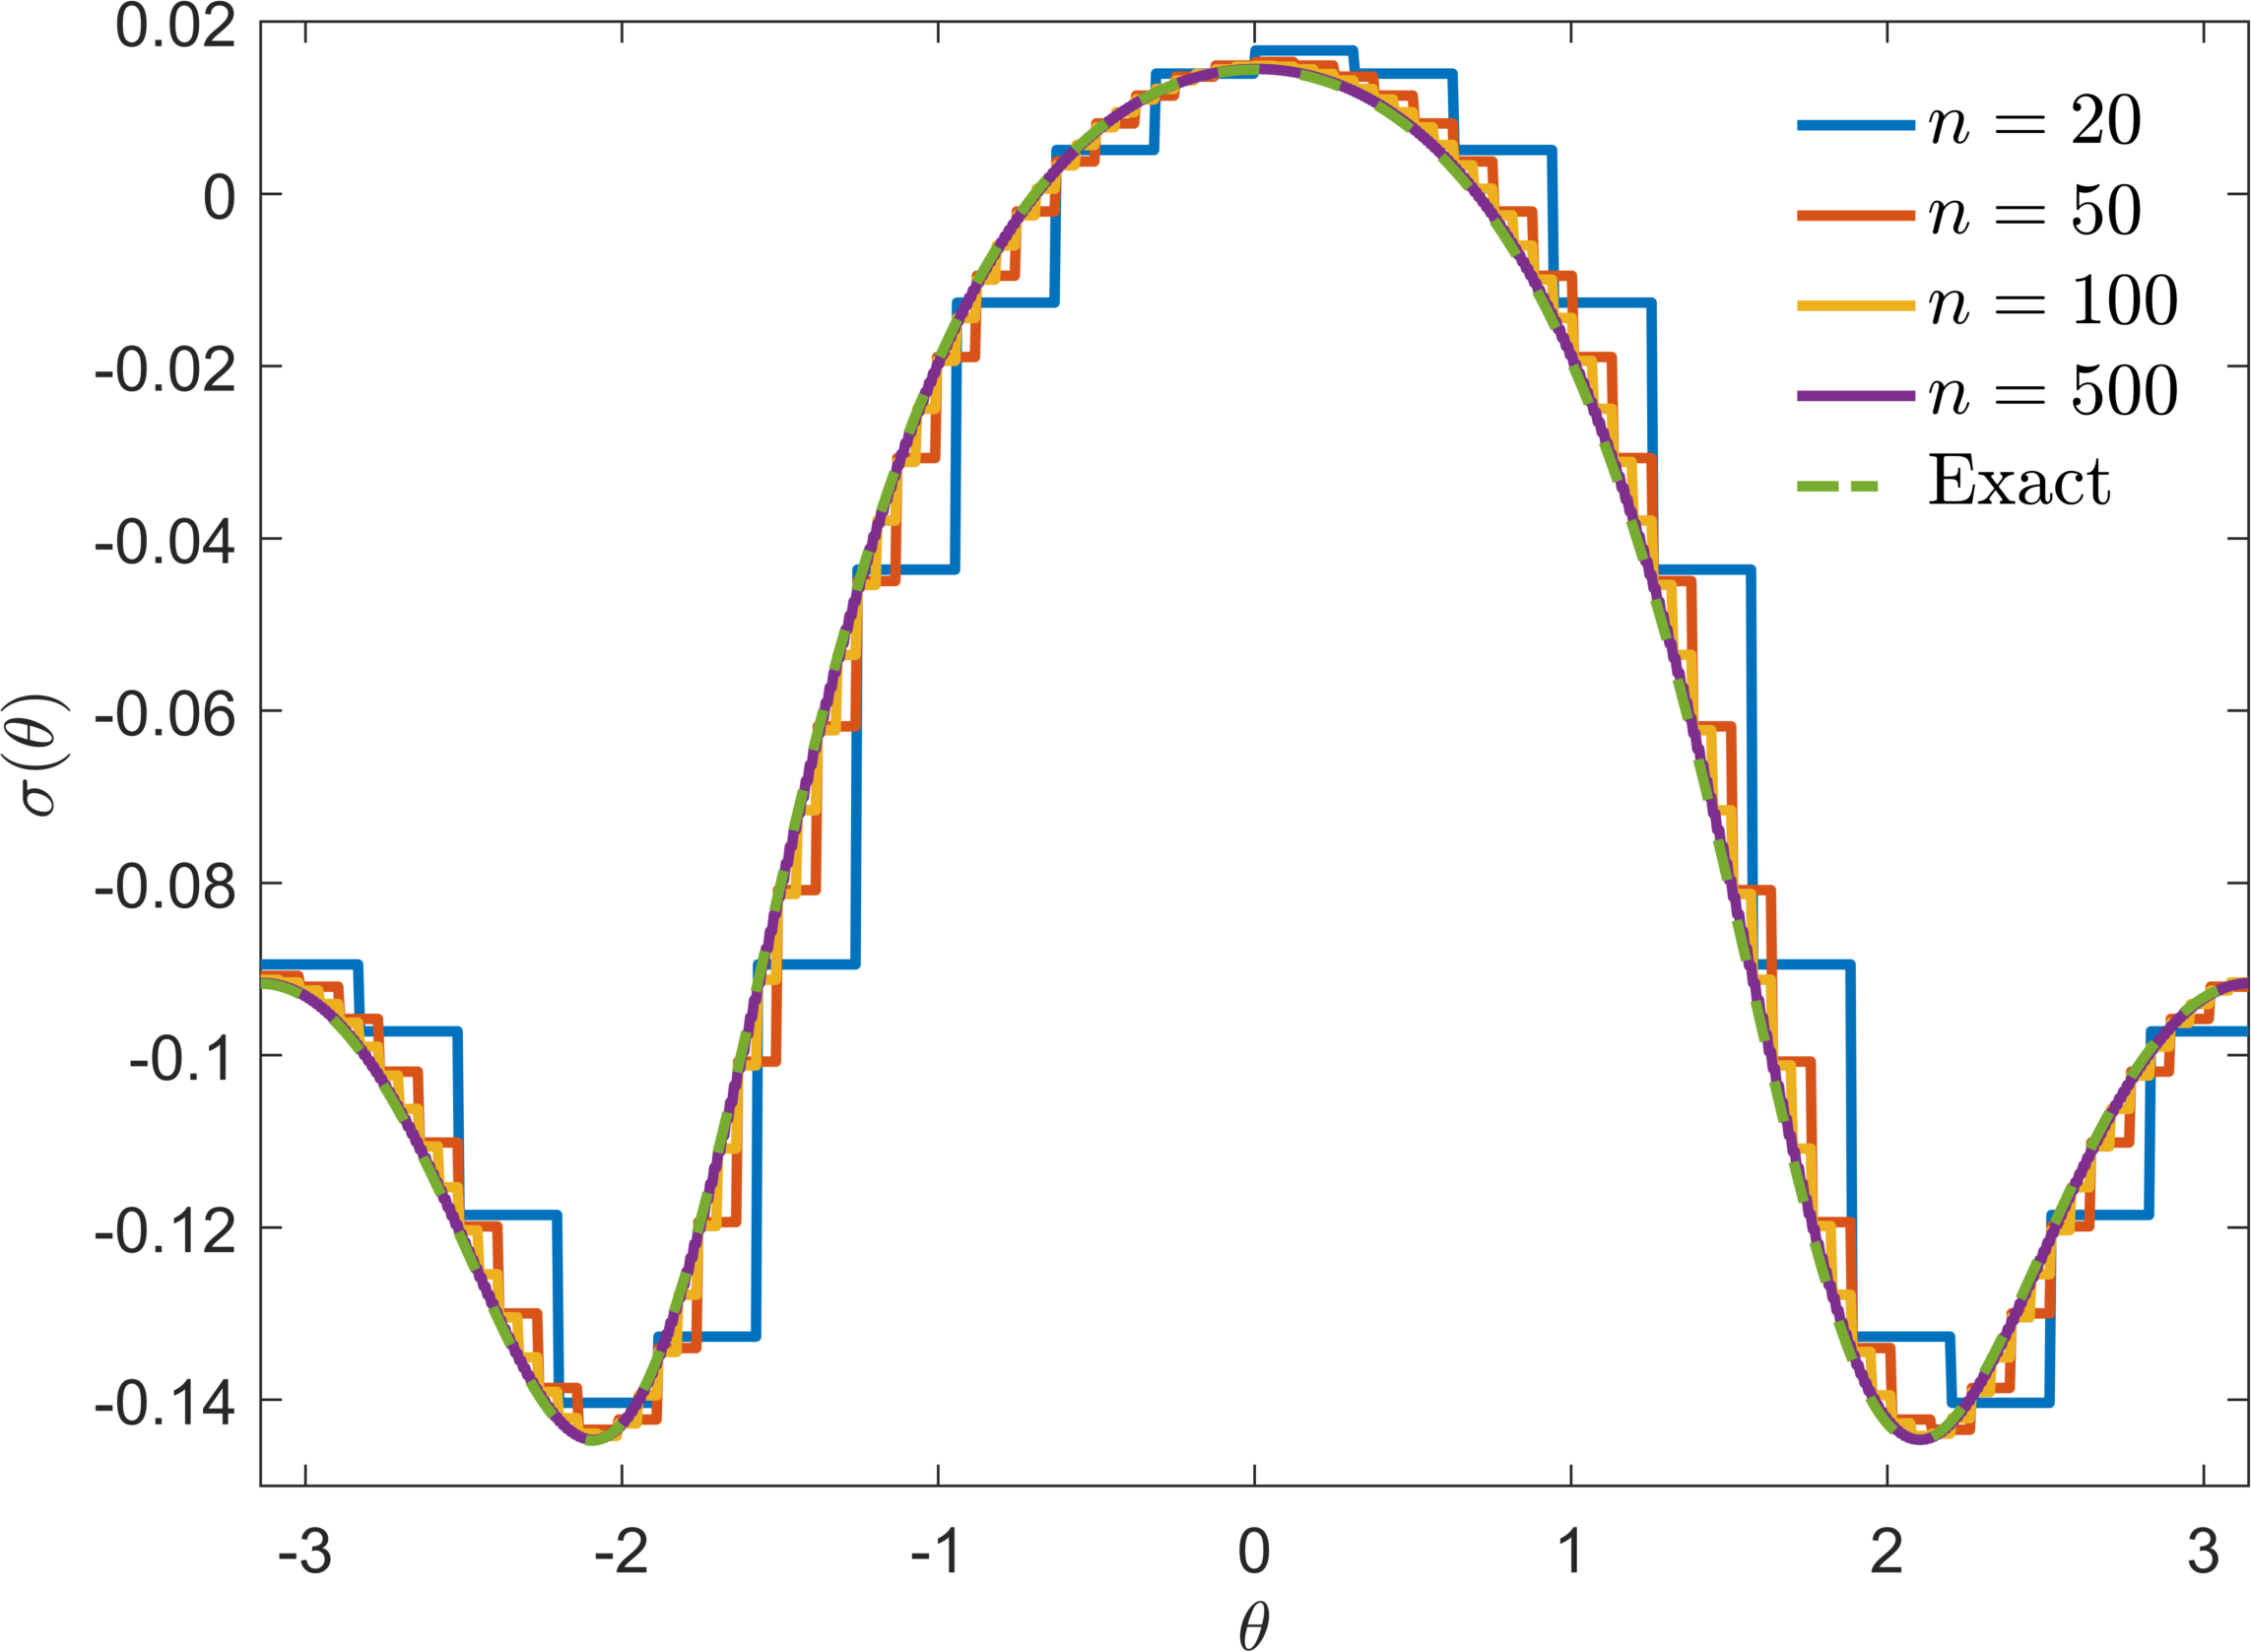
\includegraphics[width=\linewidth]{sigma_solution.png}
  \caption{Plot of $\sigma(\theta)$ for various values of $n$. The exact solution is shown as a dashed green curve to allow for comparison with the approximate solutions.}
  \label{fig:sigma_solution}
\end{figure}

Figure \ref{fig:sigma_solution} shows the approximate discrete solution $\sigma_i$ for various values of $n$, with the exact solution superimposed for comparison. The approximate solution converges to the exact solution, being virtually indistinguishable when $n=500$. Actually, if each point was connected with a straight line, the solution at $n=50$ would have been indistinguishable from the exact solution.

\subsection{Error analysis}
We can repeatedly solve the problem for $\sigma_i$ for various values of $n$ and compute the error between the approximate and exact solutions for each value of $n$. The error is calculated using
\begin{equation*}
  e_n = \sumop_{i=1}^n \lvert \sigma_i - \sigma(\theta_i) \rvert
\end{equation*}
where $\sigma_i$ is the approximate solution at $\bm{x}_i$ and $\sigma(\theta_i)$ is the exact solution evaluated at $\bm{x}_i = (\cos\theta_i, \sin\theta_i)$.

\begin{figure}[!htb]
  \centering
  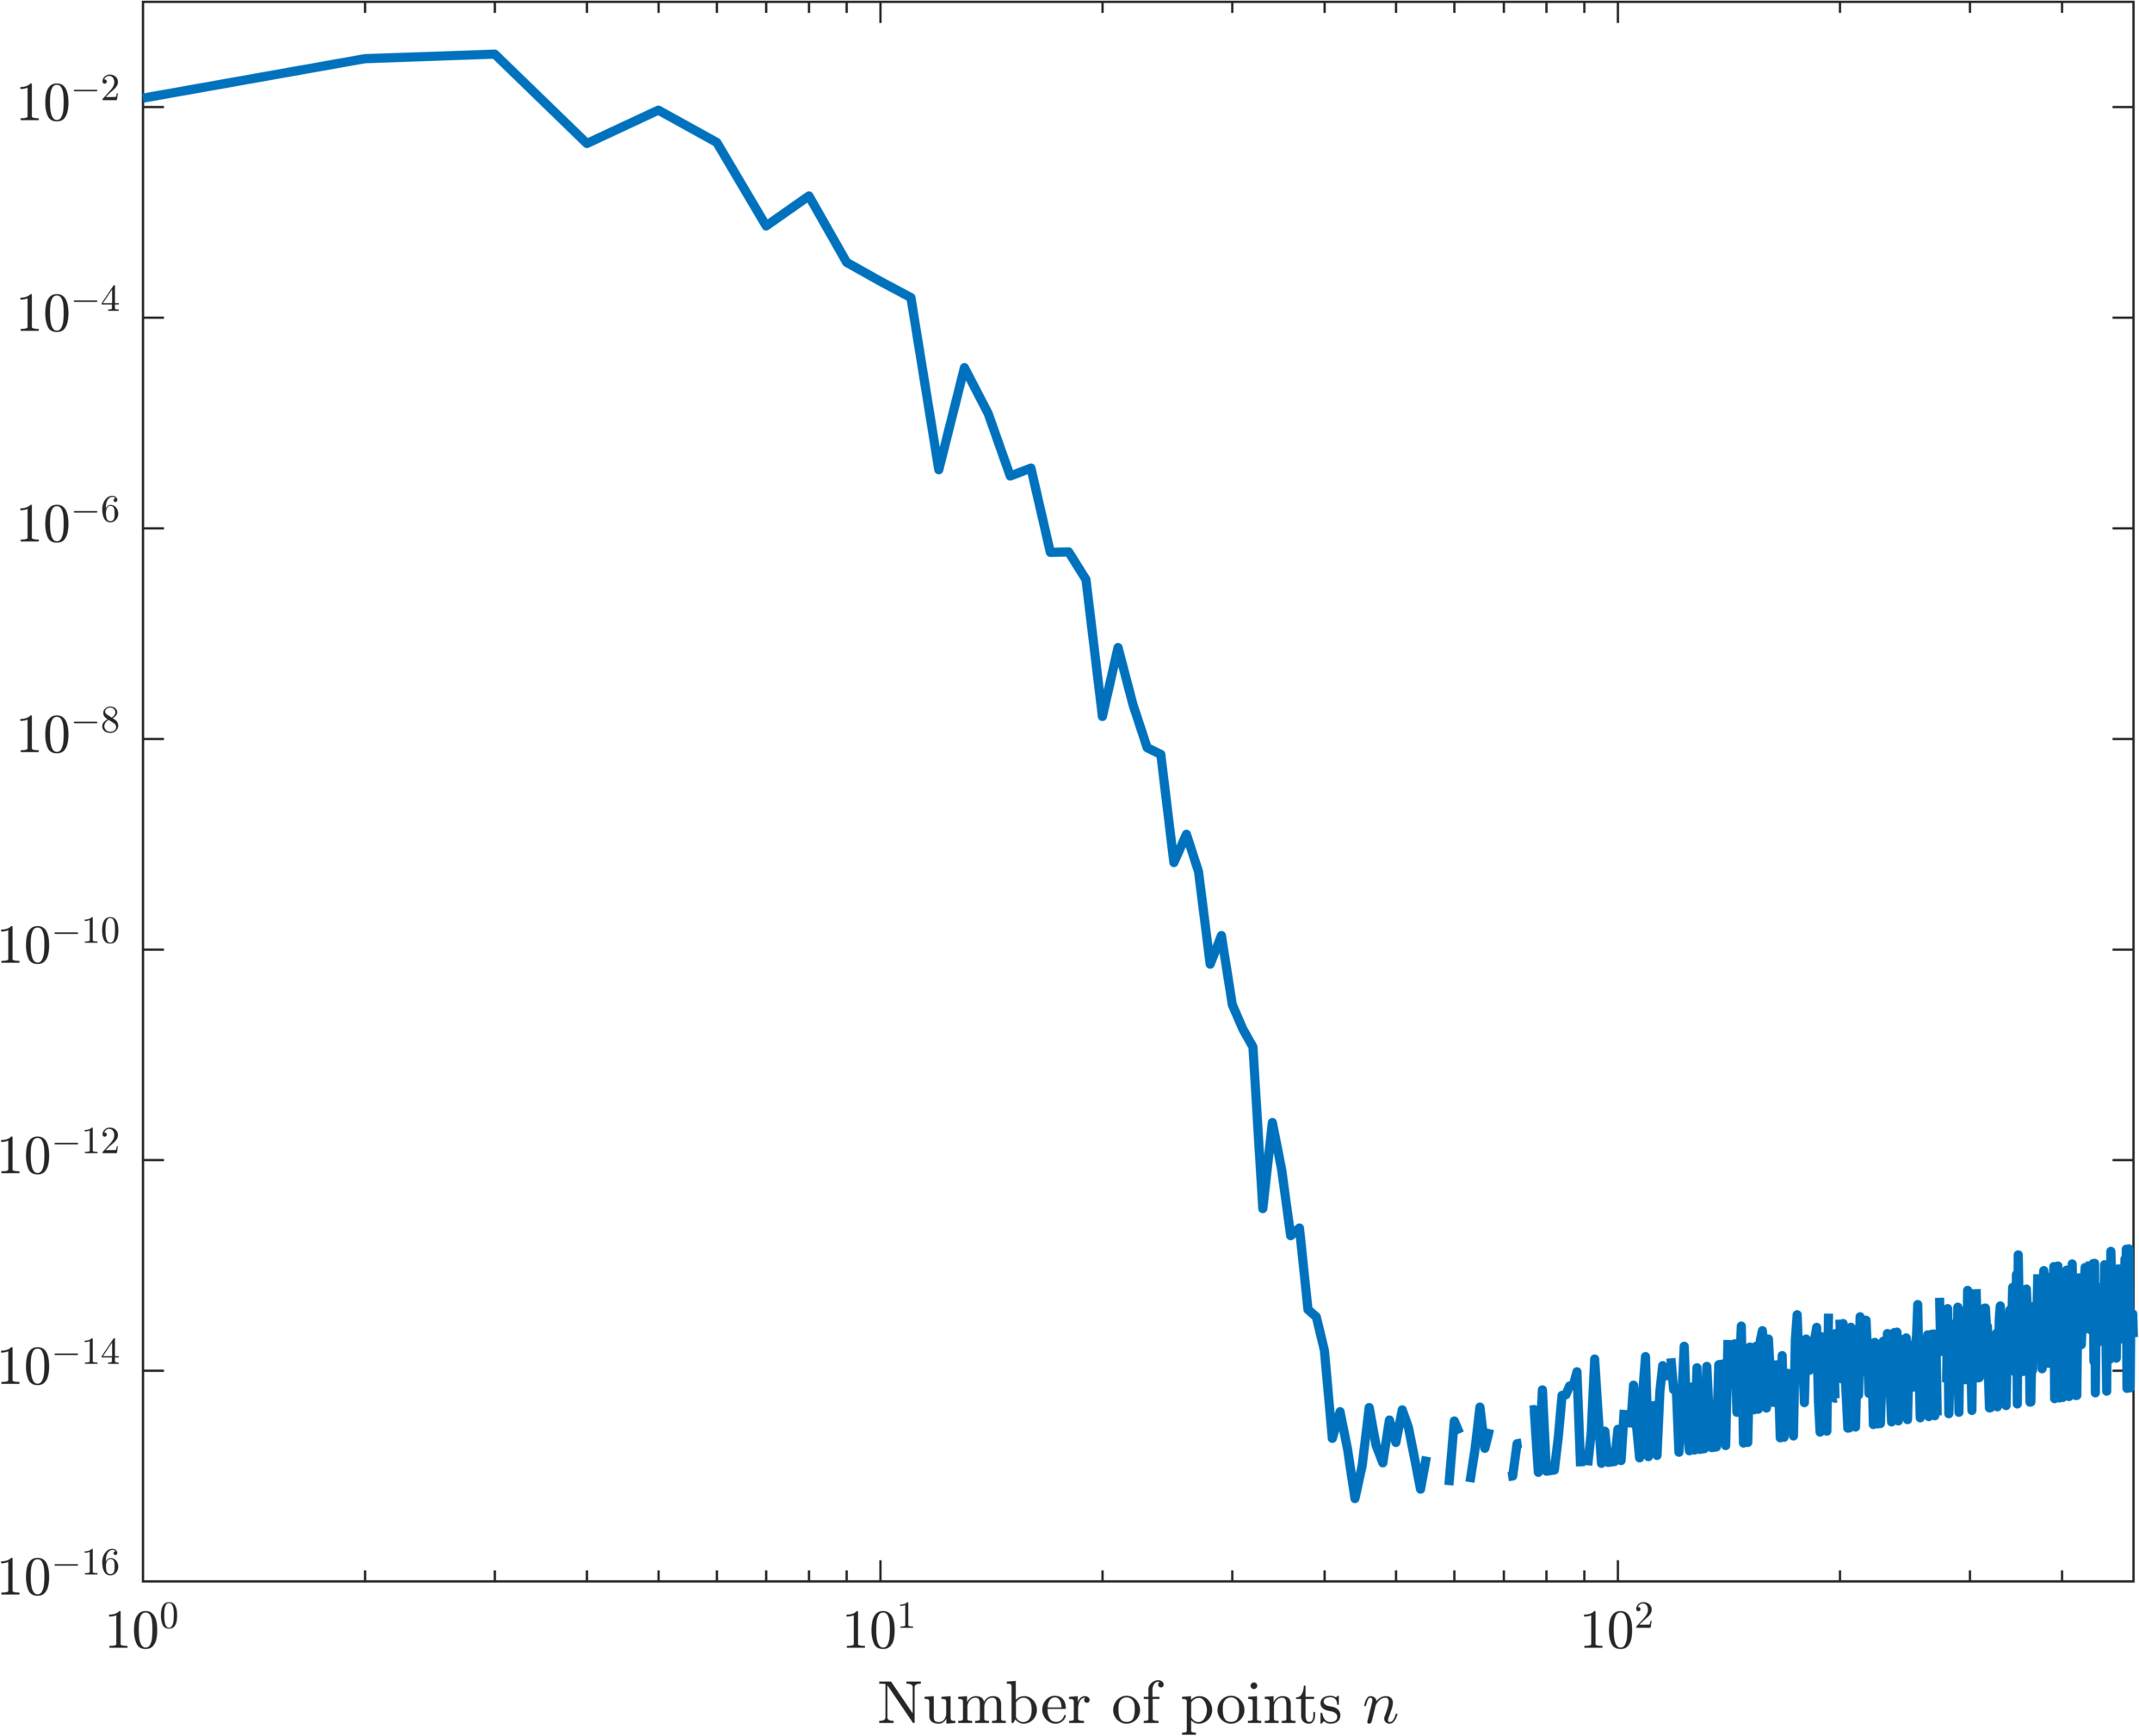
\includegraphics[width=0.9\linewidth]{sigma_error.png}
  \caption{The absolute error in the approximate solution $\bm{\sigma}_n$ compared to the exact value. Some data points appear to be missing at values of $n$ that result in zero error due to the value of $\log 0$ being undefined. (Note: the $y$-axis should be labeled ``absolute error''.)}
  \label{fig:sigma_error}
\end{figure}

Figure \ref{fig:sigma_error} shows the absolute error $e_n$ as a function of the number of points $n$. We see that in this particular case, we achieve exponential convergence, nearing machine epsilon precision at around $n=40$. It seems that the error increases linearly beyond that point, possibly due to an accumulation of many small errors, each of which are near machine epsilon.

\subsection{Solving the interior Neumann problem}
In attempting to solve the interior Neumann problem with the same boundary $\Gamma$ and Neumann boundary condition,
\begin{equation}
\p{u_\Gamma(\bm{x})}{\bm{n}}
= +\pi\sigma(\bm{x}) - \mathrm{P.V.}\int_\Gamma \frac{\bm{x-x'}}{\norm{\bm{x-x'}}^2} \cdot \bm{n}(\bm{x}) \, \sigma(\bm{x}') \, d\Gamma'
\end{equation}
we a get an almost identical system of linear equations
\begin{equation*}
\frac{1}{3 + 2\cos\theta_i + \cos(2\theta_i)}
= +\pi\sigma_i - \sumop_{j=1}^n \frac{\pi}{n} \sigma_j \, , \quad i = 1,2,\dots,n
\end{equation*}
however, when the matrix of the system $A$ is assembled, we find that $\det A = 0$ and the matrix is actually singular. 

\subsection{Solving the exterior Neumann problem on an elliptical boundary}

\end{document}